%% LyX 2.1.2.2 created this file.  For more info, see http://www.lyx.org/.
%% Do not edit unless you really know what you are doing.
\documentclass[twocolumn,english]{article}
\usepackage[T1]{fontenc}
\usepackage[latin9]{inputenc}
\usepackage{geometry}
\geometry{verbose,tmargin=1in,bmargin=1in,lmargin=1in,rmargin=1in,columnsep=0.25in}
\usepackage{float}
\usepackage{graphicx}
\usepackage{babel}
\begin{document}

\title{Preliminary Submission: Numerical Modeling of Granular Salt}


\author{Brandon Lampe and Laxmi Paneru}

\maketitle

\section*{Nomenclature}

\noindent $\dot{\epsilon}=$ Strain rate

\noindent $Q_{a}=$Activation energy

\noindent $R=$ Universal gas constant

\noindent $T=$ Absolute temperature

\noindent $C_{1}=$ Constant factor


\section{Introduction}

Granular (or crushed) salt is a candidate material for sealing the
Waste Isolation Pilot Plant's (WIPP) shafts, drifts, and boreholes;
therefore, the ability of crushed salt to prevent fluid migration
is of interest. The objective of our research is to better understand
the mechanical properties of crushed salt as they pertain to its transport
properties, most notably its intrinsic permeability, which will provide
a direct measure of its adequacy as a sealing material. Because a
materials permeability is directly related to the pore volume of the
material (along with connectivity of the pores), we are currently
focusing on the ability of a constitutive model to accurately predict
volumetric strain. In a effort to complete this objective, we have
performed a suite of laboratory tests on crushed salt over a variety
of conditions and have measured it's transient deformation.

The following sections will first familiarize the reader with existing
constitutive models. Then a description of typical test methods and
results are presented. A brief description of the currently employed
constitutive models is provided followed by the model description
and results. We will compare the results of different constitutive
models to our measured data and quantify the ability of these models
to predict the measured strain values. 


\section{Literature Review}

Mechanical properties of in situ salt were first well characterized
by Munson and Dawson during the early 1970's\cite{Munson1979}, where
they first utilized an Arrhenius type equation to describe the time
dependent deformation of salt, which is now common practice, this
relationship is shown below: 
\[
\dot{\epsilon}=C_{1}*exp\Bigg(\frac{-Q_{a}}{RT}\Bigg)
\]
 

During that same period, crushed salt became of interest to the engineering
community also, predominately for use as a seal material around nuclear
wast packages, shafts, and other openings associated with the storage
of nuclear waste. The first recorded laboratory tests, performed for
obtaining constitutive parameters were uniaxial compression tests
completed in 1978 on samples that were 5 centimeters in diameter \cite{Hansen1976}.
However, the small specimen sizes utilized in these early tests had
nonuniform stress fields (from side and end friction) producing inconsistent
results. Since the first tests on crushed salt were performed, testing
techniques have advanced greatly and we are now able to accurately
measures strains at at high temperatures and pressures that are representative
of downhole conditions in a nuclear waste storage facility\cite{Broome2014}. 

During the last 39 years, over ten constitutive models have been developed
for crushed salt, each based on varying degrees of phenomenology,
micro mechanics, and/or empiricism\cite{Callahan1995}. During the
mid-1990's, the Crushed Salt (CS) model was developed, with funding
from the US Dept. of Energy, which was the first model to combine
several dominant deformation attributes of crushed salt, such as grain
boundary pressure solutioning and dislocation creep, which are believed
to be dominant deformation mechanisms of crushed salt \cite{Spiers1993,Zeuch1990,Callahan1998IJRM}.
Including these different deformation mechanisms is critical to accurately
predicting the deformation of salt, as the dominant mechanism varies
with local conditions\cite{Frost1982}. The CS model has the ability
to predict the deformation of crushed salt reasonably well at low
temperatures, but at high temperatures Broome et al. \cite{Broome2014}
showed the model predictions did not well represent the true deformations.
An additional shortcoming of the CS model is the large number of material
parameters (constants) associated with it, 31 independent parameters
in total, which produce a highly nonlinear result that makes fitting
parameters to a specific salt deposit very difficult. The US Dept.
of Energy currently utilizes the CS model to aid in there planning
and development of storage facilities; therefore this model is of
particular interest to us. 

More recently, Olivella and Gens \cite{Olivella2002} developed an
additional constitutive model that utilizes a nonlinear viscous approach
that again focused on capturing the deformation associated with the
active deformation mechanisms at different conditions. This model
is currently employed by the THERESA project, which is a European
based group aimed at developing, verifying and improving the modeling
capabilities associated with the storage of nuclear waste. We do not
currently have access to this model; therefore, this model will not
be analyzed at this time.


\section{Test Methods and Results}

The laboratory data was obtained during a hydrostatic and shear compression
tests of a crushed salt, approximate specimen geometry is shown in
Figure\ref{fig:Sample}. Axial displacements were measured via linear
variable differential transformers (LVDTs) placed external to the
specimen, lateral displacements were measured with a pair of Shuler
gages placed circumferentially around the specimen, and metering of
the confining fluid volume. Results from the measured strains are
shown in Figure \ref{fig:StrainMeas} along with the resulting reduction
in porosity shown in Figure \ref{fig:PorosityMeas}.

\begin{figure}[h]
\begin{centering}
\includegraphics[height=7cm]{TriaxialSetup_bcl}
\par\end{centering}

\protect\caption{Representation of crushed-salt specimen in the triaxial cell.\label{fig:Sample}}
\end{figure}


\begin{figure}[h]
\begin{centering}
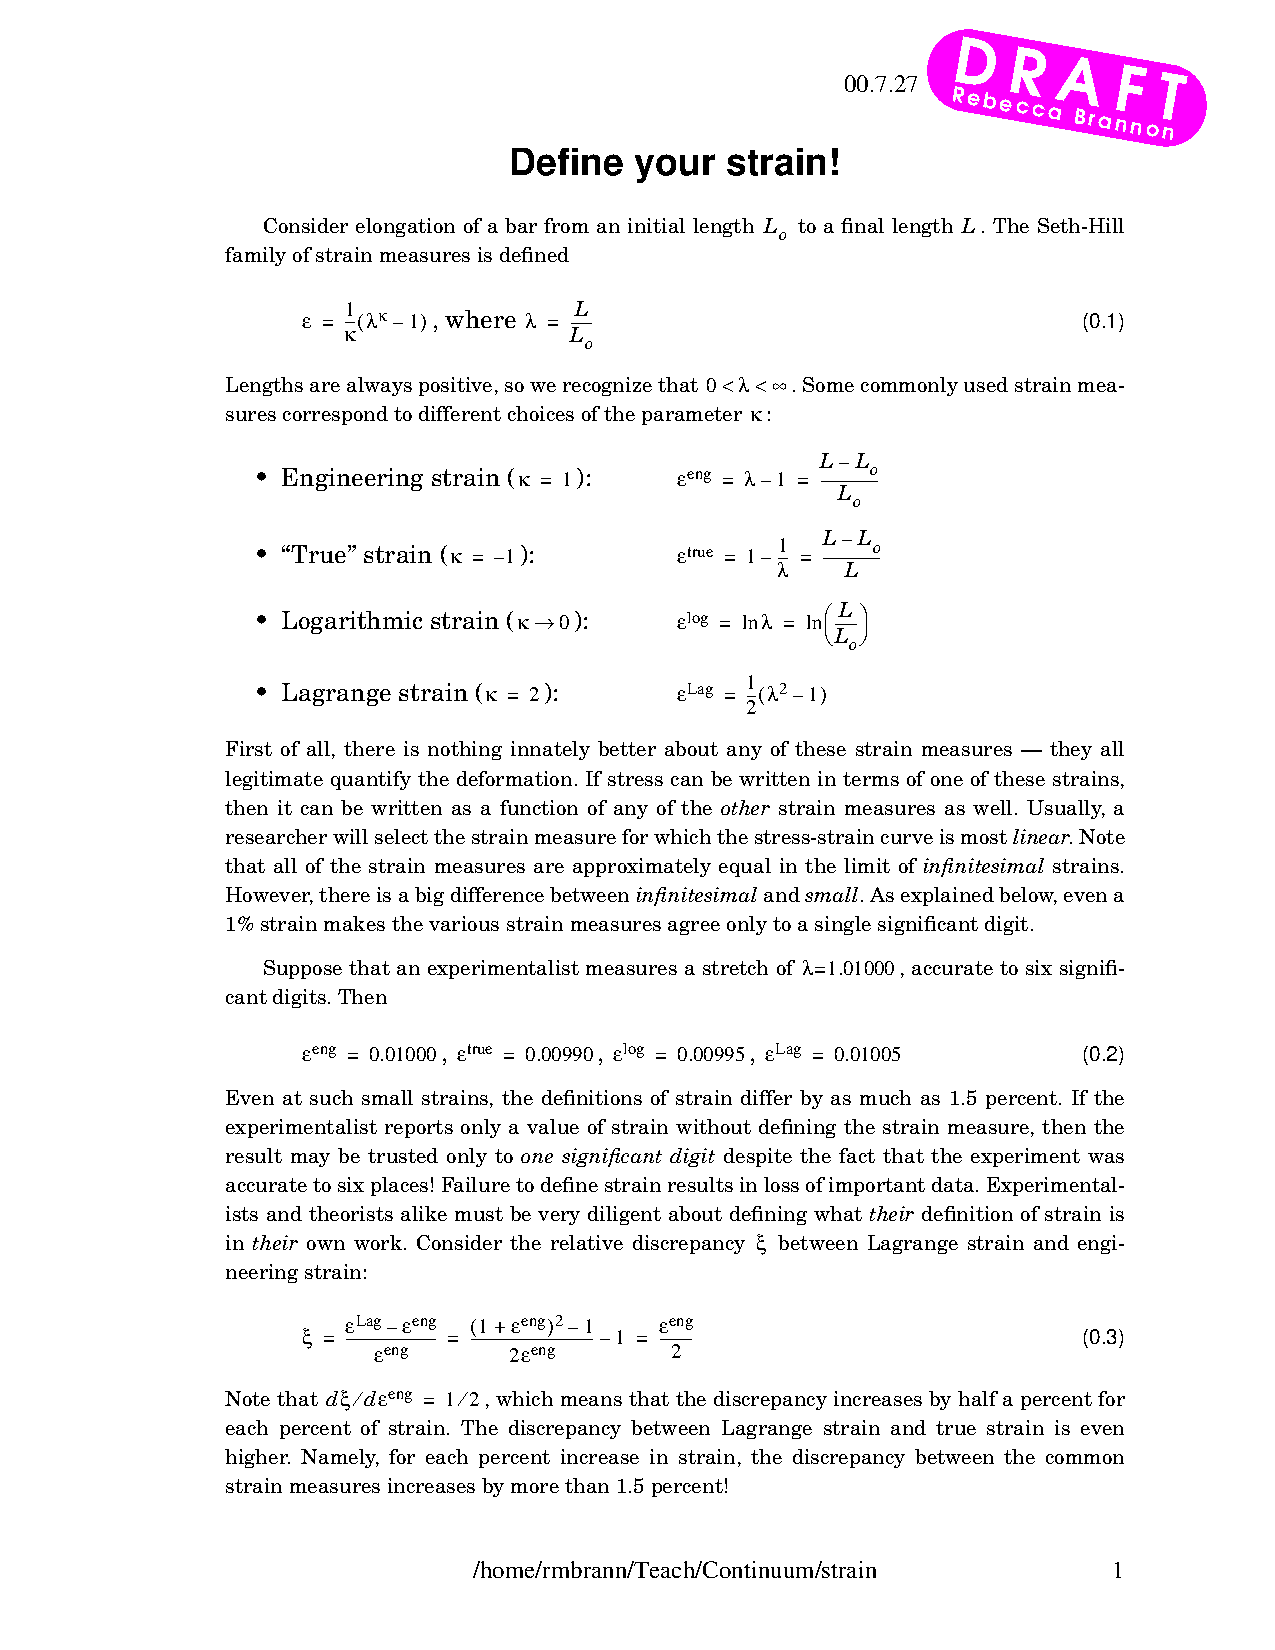
\includegraphics[width=8cm]{strain}
\par\end{centering}

\protect\caption{Strain measures during the hydrostatic compression test.\label{fig:StrainMeas} }


\end{figure}


\begin{figure}[h]
\begin{centering}
\includegraphics[width=8.5cm]{porosity}
\par\end{centering}

\protect\caption{Calculated porosity during a hydrostatic compression test.\label{fig:PorosityMeas}}


\end{figure}



\section{Constitutive Models}

We plan to predict the deformation measured during laboratory tests
using the following constitutive models:
\begin{itemize}
\item Generalized Hooke's law for linear elasticity
\item Drucker-Prager/cap plasticity
\item CS Model
\end{itemize}
The first two constitutive models may be implemented using Abaqus
once the material parameters are obtained from tests data. However,
Abaqus does not contain the CS model in its library, but we wish to
compare results of the CS model to other existing models\cite{Abaqus2012}.
Therefore, we have programmed the CS model in the R language, and
our algorithm produces the predicted strains from the CS model. This
implementation of the CS model allows for the comparisons with other
constitutive models in the Abaqus library when a single element is
utilized.


\section{Model Description}

Numerical analyses were performed using the program Abaqus/CAE 6.14-1
to perform the finite element analyses. Abaqus contains a range of
constitutive models and elements to choose from. Currently, our finite
element model contains 1,566 nodes and 1170 8-node brick elements.
We plan on complete multiple meshes of our model with both less and
more elements to determine how many elements are needed for convergence
of a solution.

Our model geometry consists of two end platens modeled as linear elastic
aluminum and the test specimen, which is ({*}will be) be modeled as
both an elastic and viscoplastic material. The test specimen was assumed
to contain two orthogonal planes of symmetry, each with essential
boundary conditions (zero displacement). The upper platen was also
defined with an essential boundary condition of zero displacement.
The lower platen and the curved face of the specimen were both defined
as having natural boundary conditions (prescribed force). The boundary
condition on the curved face of the specimen were defined as a constant
pressure (no shear component) that represents the confining fluid.
Additionally, the lower platen was prescribed an constant pressure.
Magnitudes of the prescribed natural boundary conditions varied depending
on the simulated test scenario (e.g., were equal for hydrostatic compression
test and not equal shear compression test). Interactions between the
salt specimen and the end platens were also modeled in attempt to
capture the influence of end affects. 


\section{Numerical Results}

Very limited results have been obtained thus far, below Figures \ref{fig:fea01}
and \ref{fig:fea02} show the deformed mesh with contour plots of
the numerical results. These results were obtained from modeling a
linear elastic specimen under a hydrostatic stress of 200 pounds per
square inch (psi). These initial results verified that essential boundary
conditions are acting as intended, i.e. zero displacement at the upper
platen and across the planes of symmetry. Natural boundary conditions
also appear to be correctly implemented as the material as uniformly
deformed in and up as was expected from a linear elastic model. Frictional
affects between the platens and specimen also appear to be captured,
as the stress distribution is not radially uniform at the specimen
ends, which was expected.

\begin{figure}[h]
\begin{centering}
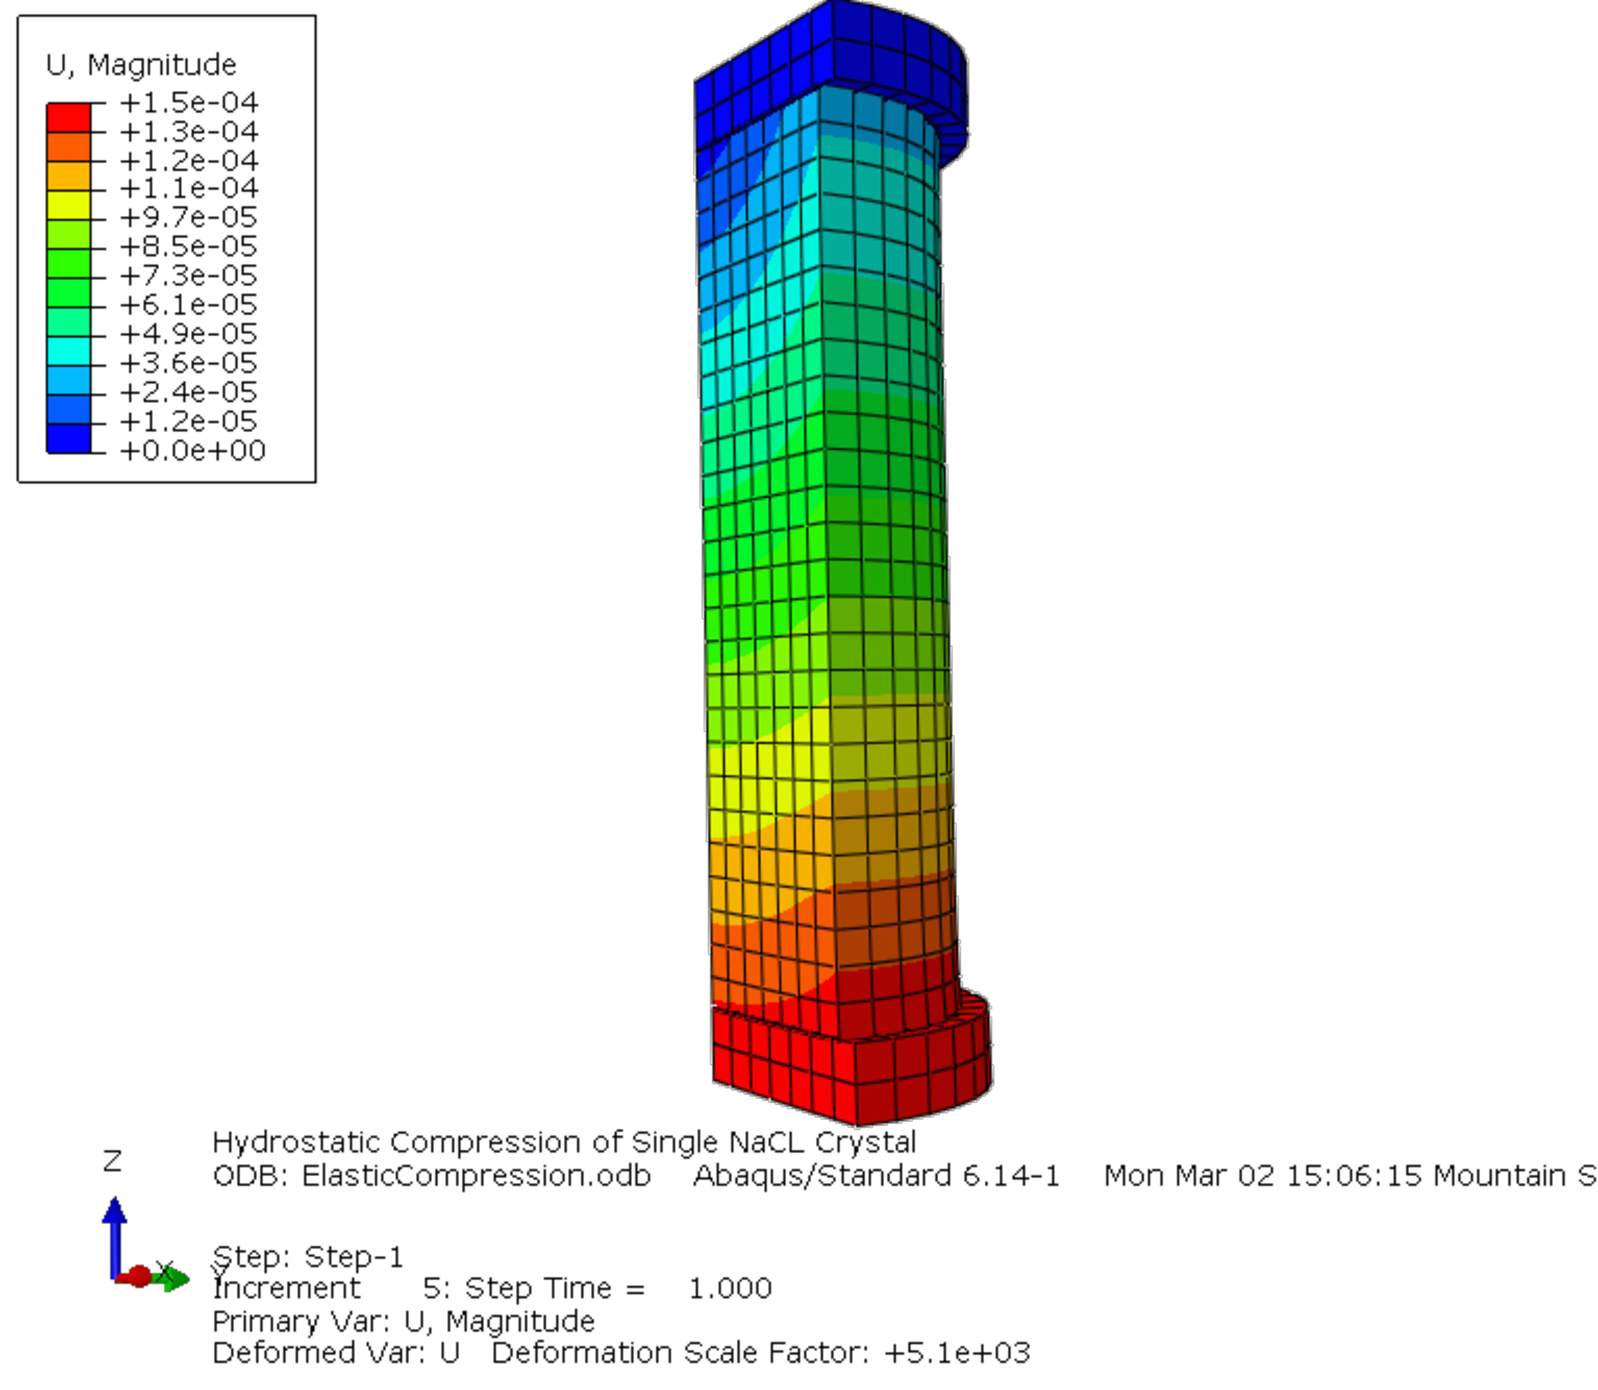
\includegraphics[width=8.25cm]{Out_ElasticDisp}
\par\end{centering}

\protect\caption{Numerical displacement (inch) results from a linear elastic simulation
performed in Abaqus.\label{fig:fea01}}


\end{figure}


\begin{figure}[H]
\begin{centering}
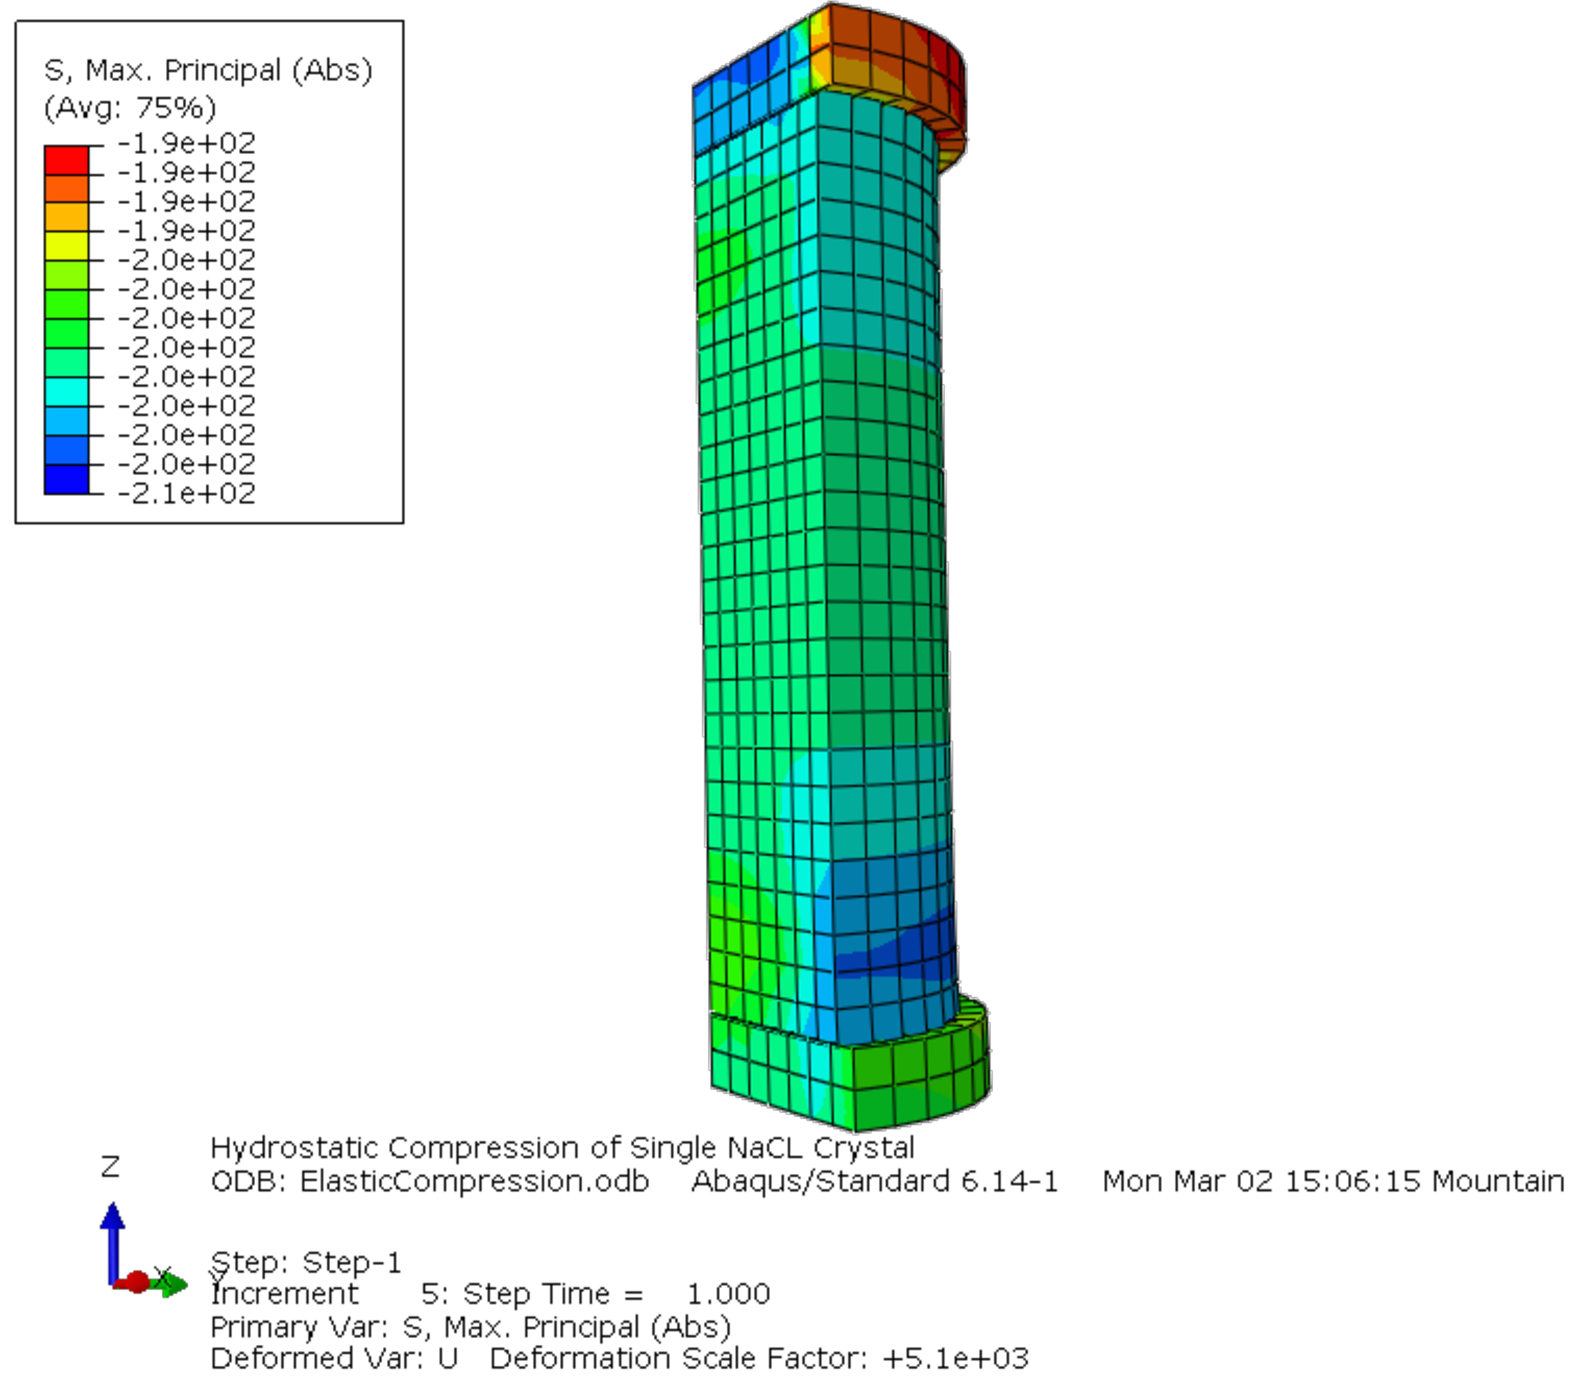
\includegraphics[width=8.25cm]{Out_ElasticStress}
\par\end{centering}

\protect\caption{Numerical stress (psi) results from a linear elastic simulation performed
in Abaqus.\label{fig:fea02}}


\end{figure}


\bibliographystyle{plain}
\bibliography{ProjectBib}

\end{document}
